\newpage
\section{Theoretical Analysis}
\label{sec:analysis}
In this section, the circuit shown in Figure~\ref{fig:Circuit} is analysed
theoretically, using the mesh method and the node method. \\
In the first one, we define a current for each elementary mesh, 
which is a loop containing no other loops, with an arbitrary direction.
These currents will be our unknown values and the objetive is to compute them, using the Ohm's Law (V = RI) and Kirchhoff Voltage Law. 
Therefore, in this circuit we wil have four currents to compute, so we have to find four equations to solve this problem. \\
\noindent In the second one, each circuit node have a defined voltage. We also choose a node to have a null voltage.
Then, we use Ohm's Law and Kirchhoff Current Law in nodes that are not connected to a voltage source.
In the end, we write additional equations for the nodes related by voltage sources.
Consequently, we will have an equal number of nodes and equations.
To calculate the unkown voltages and currents, we use the following values (Resistances in kOhm, voltages in Volts, currents in mA, $K_b$ in S and $K_c$ in Ohms):
\begin{table}[h!]
\centering
\begin{small}
\caption{Given values.} \label{Table1}
\begin{tabular}{c|c}
\hline
$R_1$ & 1,00332071212 \\
$R_2$  & 2,04460853047 \\
$R_3$  & 3,08291730437 \\
$R_4$ & 4,16061678649 \\
$R_5$  & 3,04022345043 \\
$R_6$ & 2,06711403452 \\
$R_7$ & 1,03302701196 \\
$V_a$ & 5,13988034104\\
$I_d$ & 1,02475824097 \\
$K_b$ & 7,0544535009 x $10^{-3}$ \\
$K_c$ & 8,16113797582 x $10^3$\\
\hline
\end{tabular}
\end{small}
\end{table}

\newpage

\section{Mesh method}
\begin{figure}[h] \centering
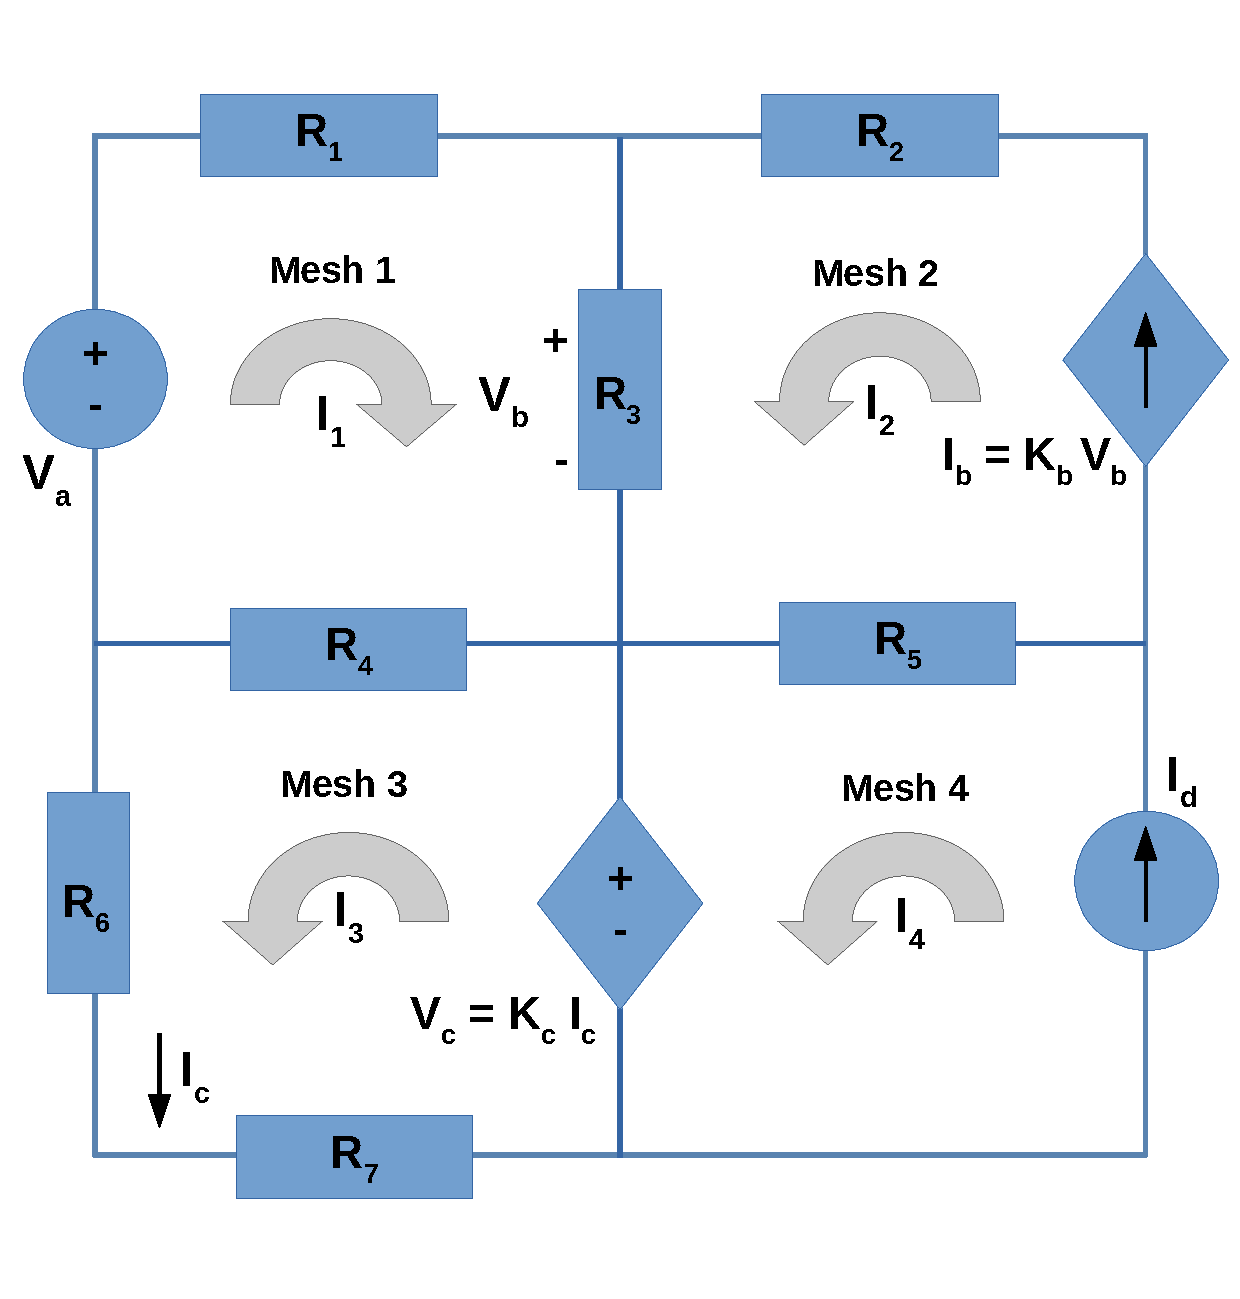
\includegraphics[width=0.6\linewidth]{Circuit_Mesh.pdf}
\caption{Circuit with current defined in each mesh.}
\label{fig:Circuit_Mesh}
\end{figure}
\noindent In Figure~\ref{fig:Circuit_Mesh}, we defined a current for each circuit essencial loop.
As said before, we will have four equations, because we need to compute four currents
($I_1$, $I_2$, $I_3$ and $I_4$).
In this analysis, we assumed that the current in mesh one is flowing clockwise and the three other currents are flowing in the other direction. Once we calculate the values to each current with the KVL method, we know that the negative ones are not flowing in the direction we assumed.

\noindent Starting with mesh 3, we can see by inspection that $I_c$ = $I_3$  and that $R_3$  depends on $I_1$  and $I_3$, which have the same direction. The other 3 components depend only on $I_3$. In the voltage source, the current flows to the positive side to the negative, so it is not aligned with the direction we selected. Hence, we must consider it negative. So we have this equation:
\begin{equation}
(I_3 + I_1)R_4 + I_3R_7+I_3R_6 - K_cI_3  = 0
  \label{eq:kcl_mesh3}
\end{equation}

\noindent In circuit analysis, we always consider the current flowing from the negative side to the positive, so in mesh 1, the voltage source is not aligned with the selected direction. For that reason, we consider $V_a$ negative. The current in $R_1$ depends only in $I_1$, which we can see by inspection, and $R_3$  and $R_4$  depend on two different currents with the same direction, which is positive because we assumed the clockwise direction. So we have: 
\begin{equation}
(I_1 + I_3)R_4 - V_a + R_3(I_2 + I_1)+ R_1I_1 = 0
  \label{eq:kcl_mesh1}
\end{equation}

\noindent We already have two equations, but we are going to need two additional ones, since we can not use this method in meshes with current sources. We can get these two equations by inspection of the two current sources. Starting with the dependent source $I_b$, we already  know the relation between this source and $V_b$, so we only have to write this term as a function of resistances and currents. We already wrote $V_b$ as a function of $R_3$, $I_2$ and $I_1$ at the third term of the previous equation for mesh 1. So we write it again:
\begin{equation}
I_2 = K_bR_3(I_2+I_1)
  \label{eq:kcl_mesh2}
\end{equation}

\noindent Finishing with the simplest equation, we can look at the fourth mesh to verify that:
\begin{equation}
I_4 = I_d
  \label{eq:kvl_kcl_mesh4}
\end{equation}

\noindent All these equations can be transformed in a matricial system as it is shown here:
$$ \left[ \begin{array}{cccc} R_4 & 0 & R_6 + R_4 + R_7- K_c  & 0\\
R_4 + R_3 + R_1   & R_3  &  R_4  & 0 \\
K_bR_3 & -1 + K_bR_3 & 0 & 0 \\
 0 & 0 & 0 & 1 \end{array} \right]
\left[ \begin{array}{c} I_1 \\ I_2 \\ I_3 \\ I_4\end{array} \right] = 
\left[ \begin{array}{c} 0 \\ V_a \\ 0 \\ I_d \end{array} \right] $$

\noindent Solving this system using Octave and the values given, we have obtained this values:
\begin{table}[h!]
\centering
\begin{small}
\caption{Meshes table.} \label{Table2}
\begin{tabular}{c|c}
\hline
Meshes currents & Values obtained (Ampers)\\
\hline
$I_1$           & 2,00 \\
$I_2$  & 1,50 \\
$I_3$         & 1,50 \\
$I_4$   & 3,00 \\
\hline
\end{tabular}
\end{small}
\end{table}

\noindent With this currents, we can discover node voltages and currents passing through each resistance, with the following equations, and knowing that $V_c$ = $K_c$$I_3$:

\begin{equation}
I_ b = I_2
  \label{eq: IB}
\end{equation}

\begin{equation}
I_ d = I_4
  \label{eq: I4}
\end{equation}

\begin{equation}
R_1[i] = I_1
  \label{eq: IR1}
\end{equation}

\begin{equation}
R_2[i] = I_2
  \label{eq: IR2}
\end{equation}

\begin{equation}
R_3[i] = I_1 + I_2
  \label{eq: IR3}
\end{equation}

\begin{equation}
R_4[i] = I_1 + I_3
  \label{eq: IR4}
\end{equation}

\begin{equation}
R_5[i] = I_4 - I_2
  \label{eq: IR5}
\end{equation}

\begin{equation}
R_6[i] = I_3
  \label{eq: IR6}
\end{equation}

\begin{equation}
R_7[i] = I_3
  \label{eq: IR7}
\end{equation}

\begin{equation}
V_b = \frac{I_b}{K_b}
  \label{eq: Vb}
\end{equation}

\begin{equation}
V_7 = V_c
  \label{eq: V7}
\end{equation}

\begin{equation}
V_6 = V_b + V_7
\label{eq: V6}
\end{equation}

\begin{equation}
V_5 = V_6 + R_2I_2
  \label{eq: V5}
\end{equation}

\begin{equation}
V_4 = V_7 + R_5(I_4 - I_2)
  \label{eq: V4}
\end{equation}

\begin{equation}
V_3 = R_7I_3
  \label{eq: V3}
\end{equation}

\begin{equation}
V_2 = V_3 + R_6I_2
  \label{eq: V2}
\end{equation}

\begin{equation}
V_1 = V_2 + V_a
\label{eq: V1}
\end{equation}

\newpage
\section{Node method}
\begin{figure}[h] \centering
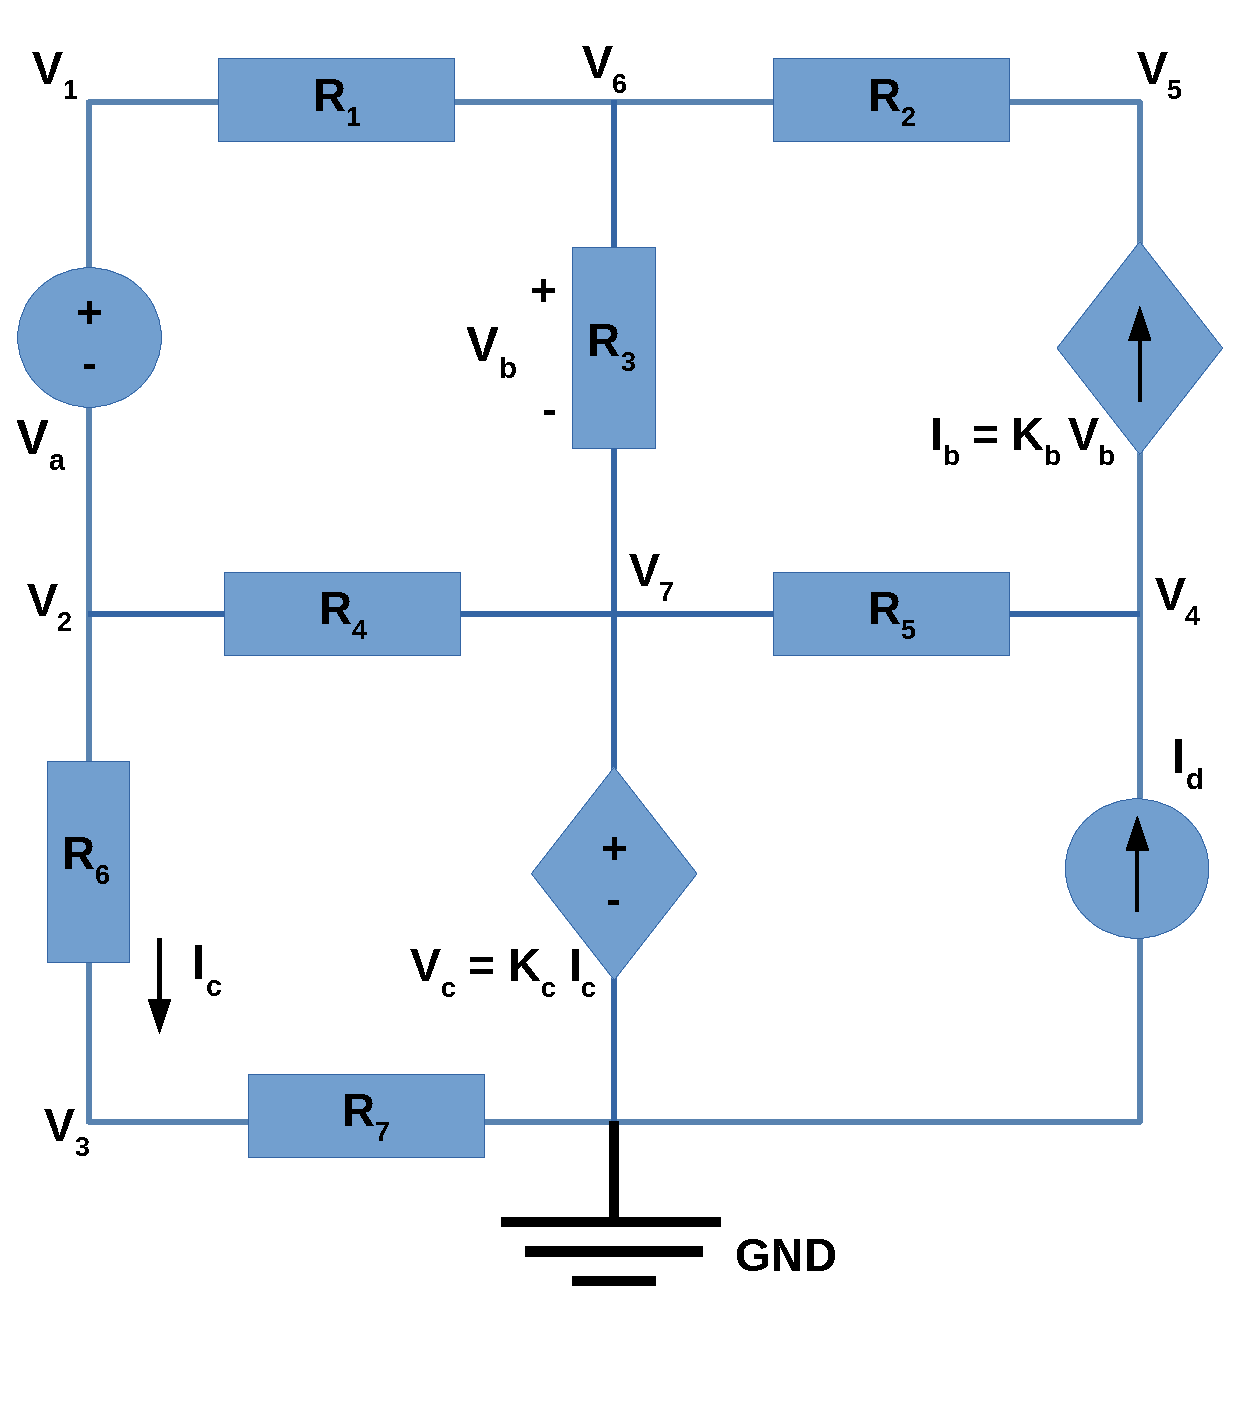
\includegraphics[width=0.6\linewidth]{Circuit_Nodes.pdf}
\caption{Circuit with voltages defined in each node.}
\label{fig:Circuit_Nodes}
\end{figure}
\noindent In Figure~\ref{fig:Circuit_Nodes}, we defined a voltage for each circuit node and a node with null voltage.
As said before, we will have seven equations, because we need to compute seven voltages 
($V_1$, $V_2$, $V_3$, $V_4$, $V_5$, $V_6$ and $V_7$).
In this analysis, we consider currents diverging from the node as positive values and currents converging as negative values, using KCL.

\noindent Starting with node 3, for this node, we considered all currents diverging, so we have this equation:
\begin{equation}
\frac{V_3 - V_2}{R_6} + \frac{V_3}{R_7} = 0
  \label{eq:kvl_node3}
\end{equation}

\noindent In node 4, only $I_d$ is converging.
$V_B$ is equal to $V_6$ - $V_7$, due to the direction represented in the circuit for $R_3$ voltage:
\begin{equation}
\frac{V_4 - V_7}{R_5} - I_d + K_b(V_6 - V_7) = 0
  \label{eq:kvl_node4}
\end{equation}

\noindent Moving on to node 5, in which only $I_b$ is converging, having this equation:
\begin{equation}
\frac{V_5 - V_6}{R_2} - K_b(V_6 - V_7) = 0
  \label{eq:kvl_node5}
\end{equation}

\noindent On the other side, in node 6, we considered all currents diverging:
\begin{equation}
\frac{V_6 - V_7}{R_3} + \frac{V_6 - V_5}{R_2} + \frac{V_6 - V_1}{R_1} = 0
  \label{eq:kvl_node6}
\end{equation}

\noindent The next equation establish the relation between nodes 1 and 2 voltages:
\begin{equation}
V_1 - V_2 = V_a
  \label{eq:kvl_node12}
\end{equation}

\noindent The relation between GND and node 7 is showed in the next equation:
\begin{equation}
V_7 = \frac{K_c(V_2 - V_3)}{R_6}
  \label{eq:kvl_node7GND}
\end{equation}

\noindent Since there is still an equation missing, we considered a super node containing $V_a$ and $R_6$ and all currents diverging:
\begin{equation}
\frac{V_1 - V_6}{R_1} + \frac{V_2 - V_7}{R_4} + \frac{V_3}{R_7} = 0
  \label{eq:kvl_supernode}
\end{equation}

\noindent All this equations can be transformed in a matricial system as it is showed here:
$$ \left[ \begin{array}{ccccccc} 0 & -\frac{1}{R_6} & \frac{1}{R_6} + \frac{1}{R_7} & 0 & 0 & 0 & 0 \\
0 & 0 & 0 & \frac{1}{R_5} & 0 & K_b & -K_b - \frac{1}{R_5} \\
0 & 0 & 0 & 0 & \frac{1}{R_2} & -K_b - \frac{1}{R_2} & K_b
\\ -\frac{1}{R_1} & 0 & 0 & 0 & -\frac{1}{R_2} & \frac{1}{R_1} + \frac{1}{R_2} + \frac{1}{R_3} & -\frac{1}{R_3}
\\ 1 & -1 & 0 & 0 & 0 & 0 & 0
\\ 0 & \frac{K_c}{R_6} & -\frac{K_c}{R_6} & 0 & 0 & 0 & -1
\\ \frac{1}{R_1} & \frac{1}{R_4} & \frac{1}{R_7} & 0 & 0 & -\frac{1}{R_1} & -\frac{1}{R_4}\end{array} \right]
\left[ \begin{array}{c} V_1 \\ V_2 \\ V_3 \\ V_4 \\ V_5 \\ V_6 \\ V_7\end{array} \right] = 
\left[ \begin{array}{c} 0 \\ I_d \\ 0 \\ 0 \\ V_a \\ 0 \\ 0\end{array} \right] $$

\noindent Solving this system using Ocatve and the values given, we have obtained this values:
\begin{table}[h!]
\centering
\begin{small}
\caption{Nodes table.} \label{Table3}
\begin{tabular}{c|c}
\hline
Nodes Voltages & Values obtained (Volts)\\
\hline
$V_1$           & 2,00 \\
$V_2$  & 1,50 \\
$V_3$         & 1,50 \\
$V_4$   & 3,00 \\
$V_5$              & 2,00 \\
$V_6$                  & 10,00 \\
$V_7$     &  7,00 \\
\hline
\end{tabular}
\end{small}
\end{table}

\noindent Having discovered nodes voltages, we need now to obtain the currents flowing in each resistance and $I_b$, with the following equations:

\begin{equation}
I_b = K_b(V_6 - V_7)
  \label{eq:Ib}
\end{equation}

\begin{equation}
R_1[i] = \frac{(V_6 - V_1)}{R_1}
  \label{eq: iR1}
\end{equation}

\begin{equation}
R_2[i] = \frac{(V_5 - V_6)}{R_2}
  \label{eq: iR2}
\end{equation}

\begin{equation}
R_3[i] = \frac{(V_6 - V_7)}{R_3}
  \label{eq: iR3}
\end{equation}

\begin{equation}
R_4[i] = \frac{(V_2 - V_7)}{R_4}
  \label{eq: iR4}
\end{equation}

\begin{equation}
R_5[i] = \frac{(V_4 - V_7)}{R_5}
  \label{eq: iR5}
\end{equation}

\begin{equation}
R_6[i] = \frac{(V_2 - V_3)}{R_6}
  \label{eq: iR6}
\end{equation}

\begin{equation}
R_7[i] = \frac{V_3}{R_7}
  \label{eq: iR7}
\end{equation}


